\documentclass[10pt]{article}

% Preamble
\usepackage[utf8]{inputenc}
\usepackage{graphicx} 
\usepackage{amsmath} 
\usepackage{caption}
\usepackage{hyperref} 
\usepackage{xcolor} 
%\usepackage{fouriernc} %New Century Schoolbook with Fourier math



% Title page details
\title{Progetto: Age from brain Data}
\author{Marco Accerenzi}
\date{Esame del 12 Settembre 2024}




% Begin the document
\begin{document}

\maketitle

\section{Introduzione e struttura del codice}

L'obiettivo del progetto è stato sviluppare un modello di regressione di deep learning per predire l'età cerebrale dei pazienti dai dati di risonanza magnetica (MRI). Il modello raggiunge un errore quadratico medio (RMS) di circa 6 anni. La configurazione ottimale è costituita da un modello con 2 hidden layers e 6 nodi per strato, ottenendo le migliori performance su dati standardizzati e normalizzati.

Sono state utilizzate le seguenti librerie:

\textit{Keras} per la costruzione del modello di regressione,
\textit{Pandas} per la lettura e manipolazione dei dati forniti in formato Excel,
\textit{Matplotlib} per tracciare e visualizzare i risultati,
\textit{os} e \textit{sys} per la gestione dei percorsi e directory.
Il codice si compone di classi e script per la gestione completa del flusso dati e la modellazione:

\textbf{ExcelData}: legge il file Excel e prepara i dati per il modello,
\textbf{RegressionModel}: implementa il modello e i metodi per addestrare, salvare e caricare il modello,
\textbf{Console}: offre un'interfaccia utente semplice per l'addestramento e la predizione,
\textbf{Optimizator}: permette la scelta rapida degli iperparametri,
\textbf{Analysis}: automatizza l'analisi dei risultati delle predizioni.
\section{Estrazione e manipolazione dei dati}

I dati MRI sono forniti in due file Excel con 915 campioni. Ogni campione contiene informazioni sull'età reale e il gruppo di provenienza dei dati. La classe \textit{ExcelData} utilizza \textit{Pandas} per caricare i dati in un dataframe e poi li converte in array \textit{numpy} per l'input nel modello.

Prima dell'addestramento, i dati vengono mescolati per prevenire l'overfitting e i valori mancanti vengono riempiti con il valore -9999. Successivamente, i dati vengono normalizzati, ovvero ogni valore è diviso per il massimo della sua colonna. Le celle con valore -9999 vengono escluse dai calcoli. La normalizzazione e la standardizzazione riducono i tempi di addestramento e migliorano la precisione delle previsioni, come mostrato in \autoref{historyNormalised} e \autoref{historyNonNormalised}.


\begin{figure}
	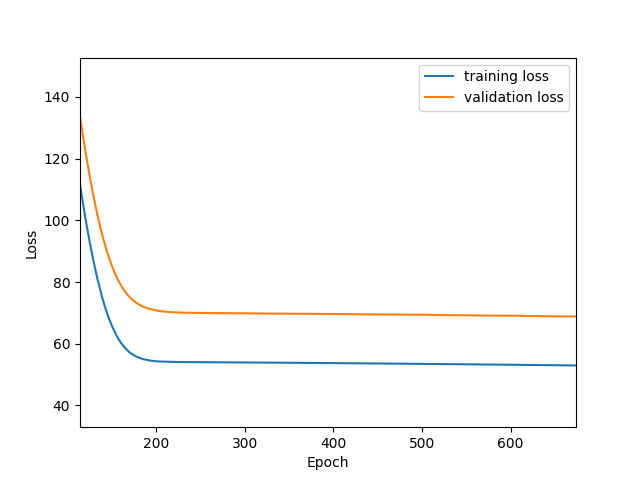
\includegraphics[width=0.8\textwidth]{Figure_2.png}
	\captionof{figure}{Grafico delle prime epoche di addestramento utilizzando dati normalizzati.}
	\label{historyNormalised}
\end{figure}

\begin{figure}
	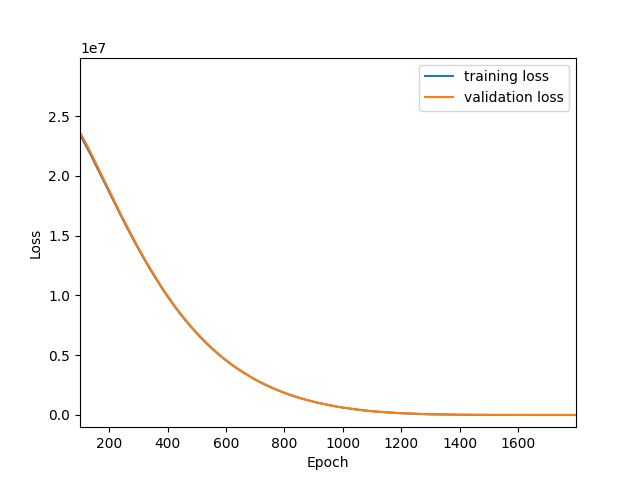
\includegraphics[width=0.8\textwidth]{History_subplot_1.png}
	\captionof{figure}{Grafico delle prime epoche di addestramento utilizzando dati grezzi.}
	\label{historyNonNormalised}
\end{figure}

\begin{figure}
	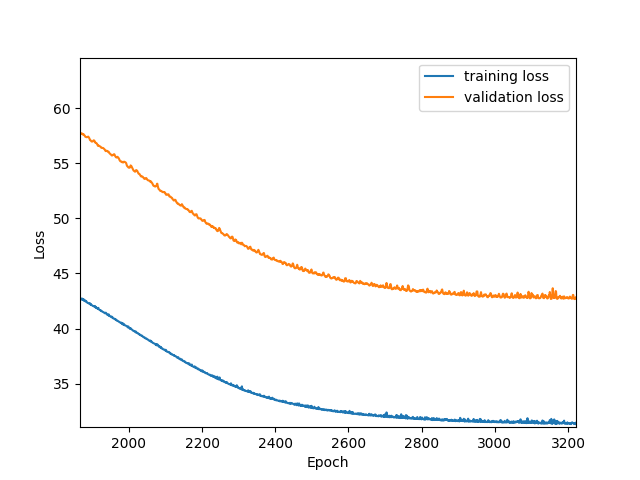
\includegraphics[width=0.8\textwidth]{Figure_4.png}
	\captionof{figure}{Grafico delle ultime epoche di addestramento utilizzando dati normalizzati.}
	\label{historyNormalised2}
\end{figure}

\begin{figure}
	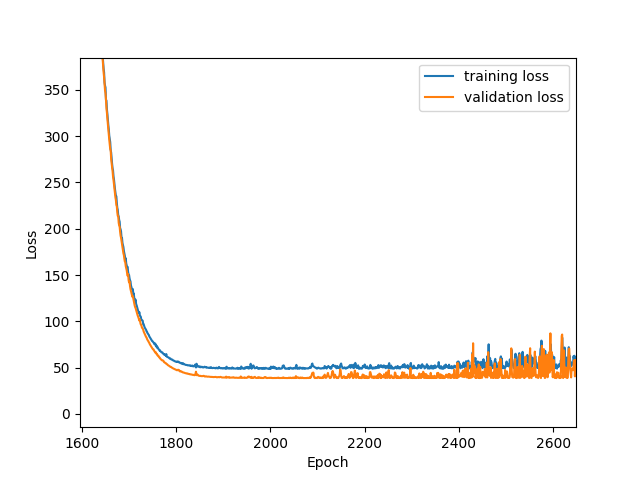
\includegraphics[width=0.8\textwidth]{History_subplot_3.png}
	\captionof{figure}{Grafico delle ultime epoche di addestramento utilizzando dati grezzi.}
	\label{historyNonNormalised2}
\end{figure}

\section{Il regression model}

Il modello di regressione utilizza i moduli \textit{models}, \textit{layers} e \textit{callbacks} di \textit{keras}. Tra i metodi implementati:

\textbf{Compile\_Model}: definisce e compila il modello,
\textbf{Start\_Training}: addestra il modello utilizzando l'algoritmo di apprendimento supervisionato,
\textbf{Plot\_History} e \textbf{Save\_Model}: salvano rispettivamente la cronologia dell'addestramento e il modello stesso,
\textbf{load\_model}: permette di caricare un modello già addestrato per l'inferenza.
Per migliorare l'efficacia dell'addestramento, vengono utilizzati i seguenti callback:

\textbf{Early stopping}: interrompe l'addestramento se la funzione di perdita non migliora dopo un certo numero di epoche, prevenendo l'overfitting,
\textbf{ModelCheckpoint}: salva checkpoint durante l'addestramento per evitare la perdita di progressi,
\textbf{ReduceLROnPlateau}: riduce il learning rate quando il modello raggiunge un plateau,
\textbf{PrintProgress}: stampa il progresso ogni n epoche.
\subsection{Ottimizzazione degli iperparametri}

Lo script \textit{Optimizator.py} è stato utilizzato per scegliere gli iperparametri. Esplora diversi valori ragionevoli degli iperparametri e realizza un addestramento breve per permettere all'utente di scegliere la configurazione ottimale. Il miglior modello è risultato avere 2 hidden layers e 6 nodi per strato, con le prestazioni migliori in termini di velocità e accuratezza.

\section{Risultati e conclusioni}

Il modello addestrato è stato utilizzato per prevedere l'età cerebrale dei pazienti, con un errore RMS costantemente tra 6.3 e 6.9 anni. Il miglior modello ha ottenuto un RMS di 6.30 anni e un MSE di 39.66. Un addestramento ripetuto potrebbe migliorare le prestazioni, ma è improbabile ottenere un RMS inferiore ai 6 anni senza incorrere in overfitting.

	\begin{figure}
		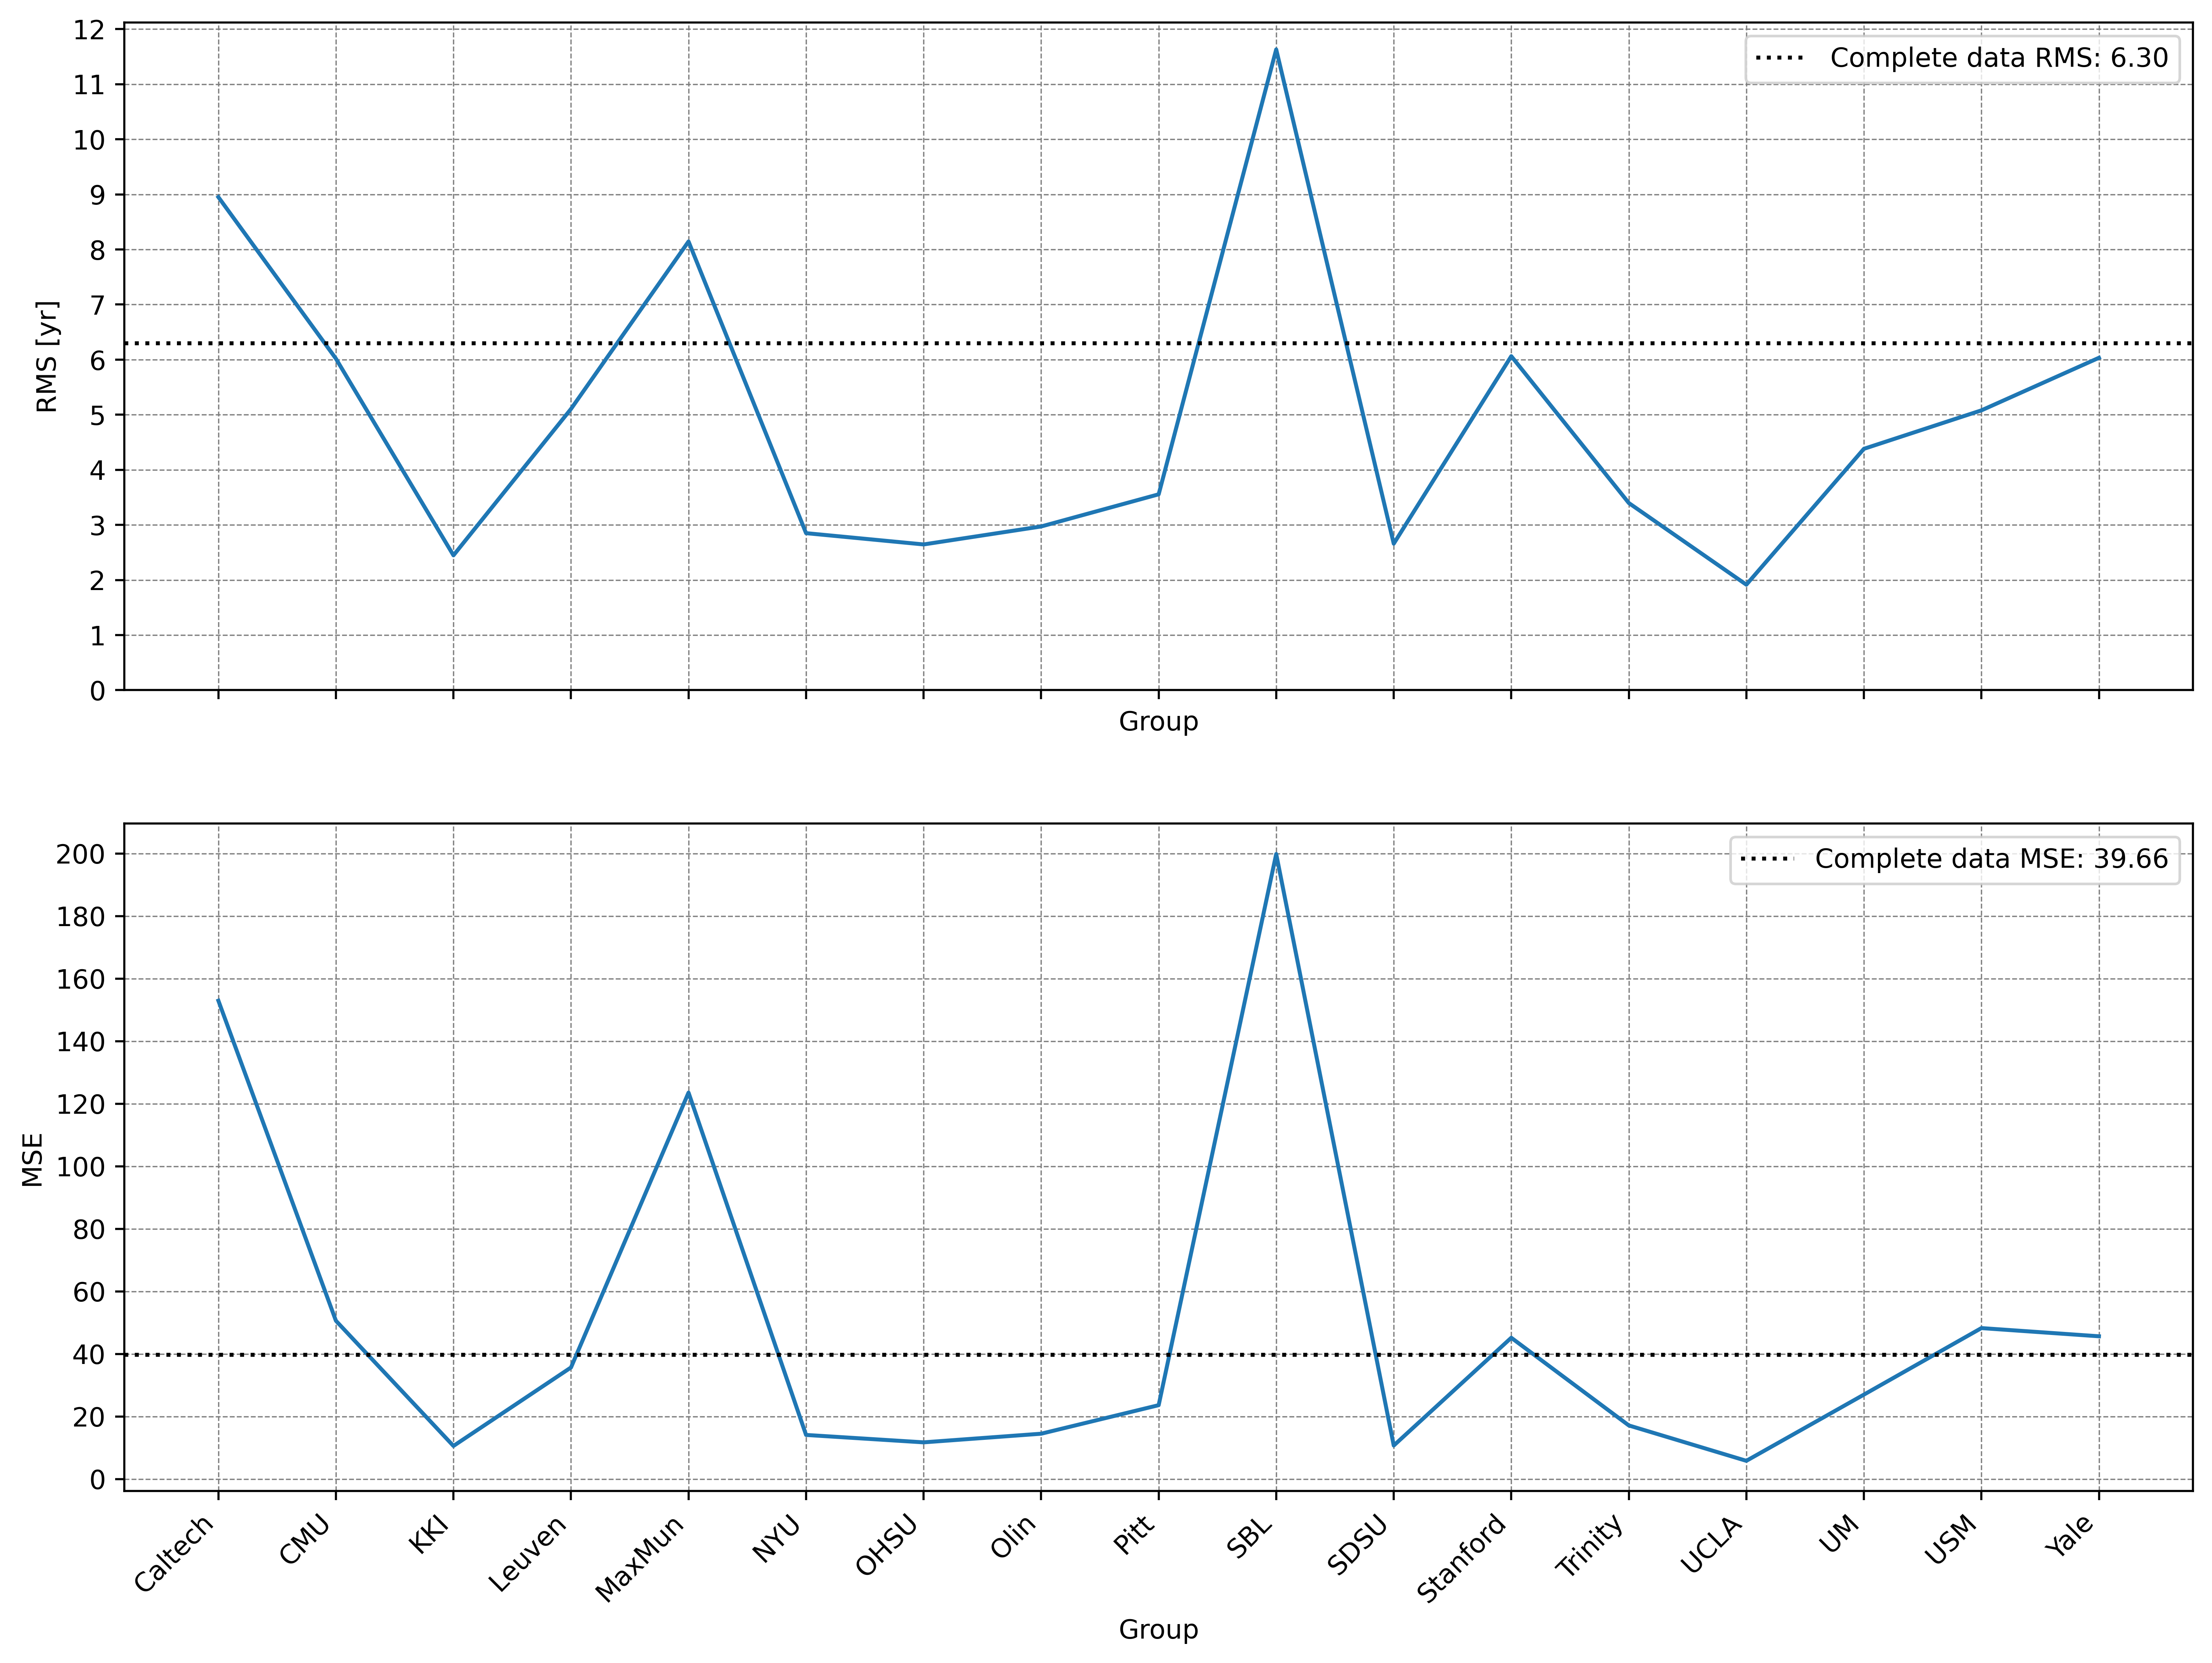
\includegraphics[width=0.8\textwidth]{result_1.png}
		\captionof{figure}{Grafico che confronta l'errore di previsione per i vari gruppi di dati. L'errore sull'intero set di dati è mostrato come una linea tratteggiata.}
		\label{plotRMSComparison2}
	\end{figure}

Il confronto tra le prestazioni dei diversi gruppi è mostrato in \autoref{plotRMSComparison2}, dove si osserva che i gruppi "Caltech", "MaxMun" e "SBL" hanno errori di predizione significativamente superiori alla media. Rimuovere questi outlier dai dati non ha migliorato sostanzialmente le prestazioni complessive del modello.


\begin{figure}
	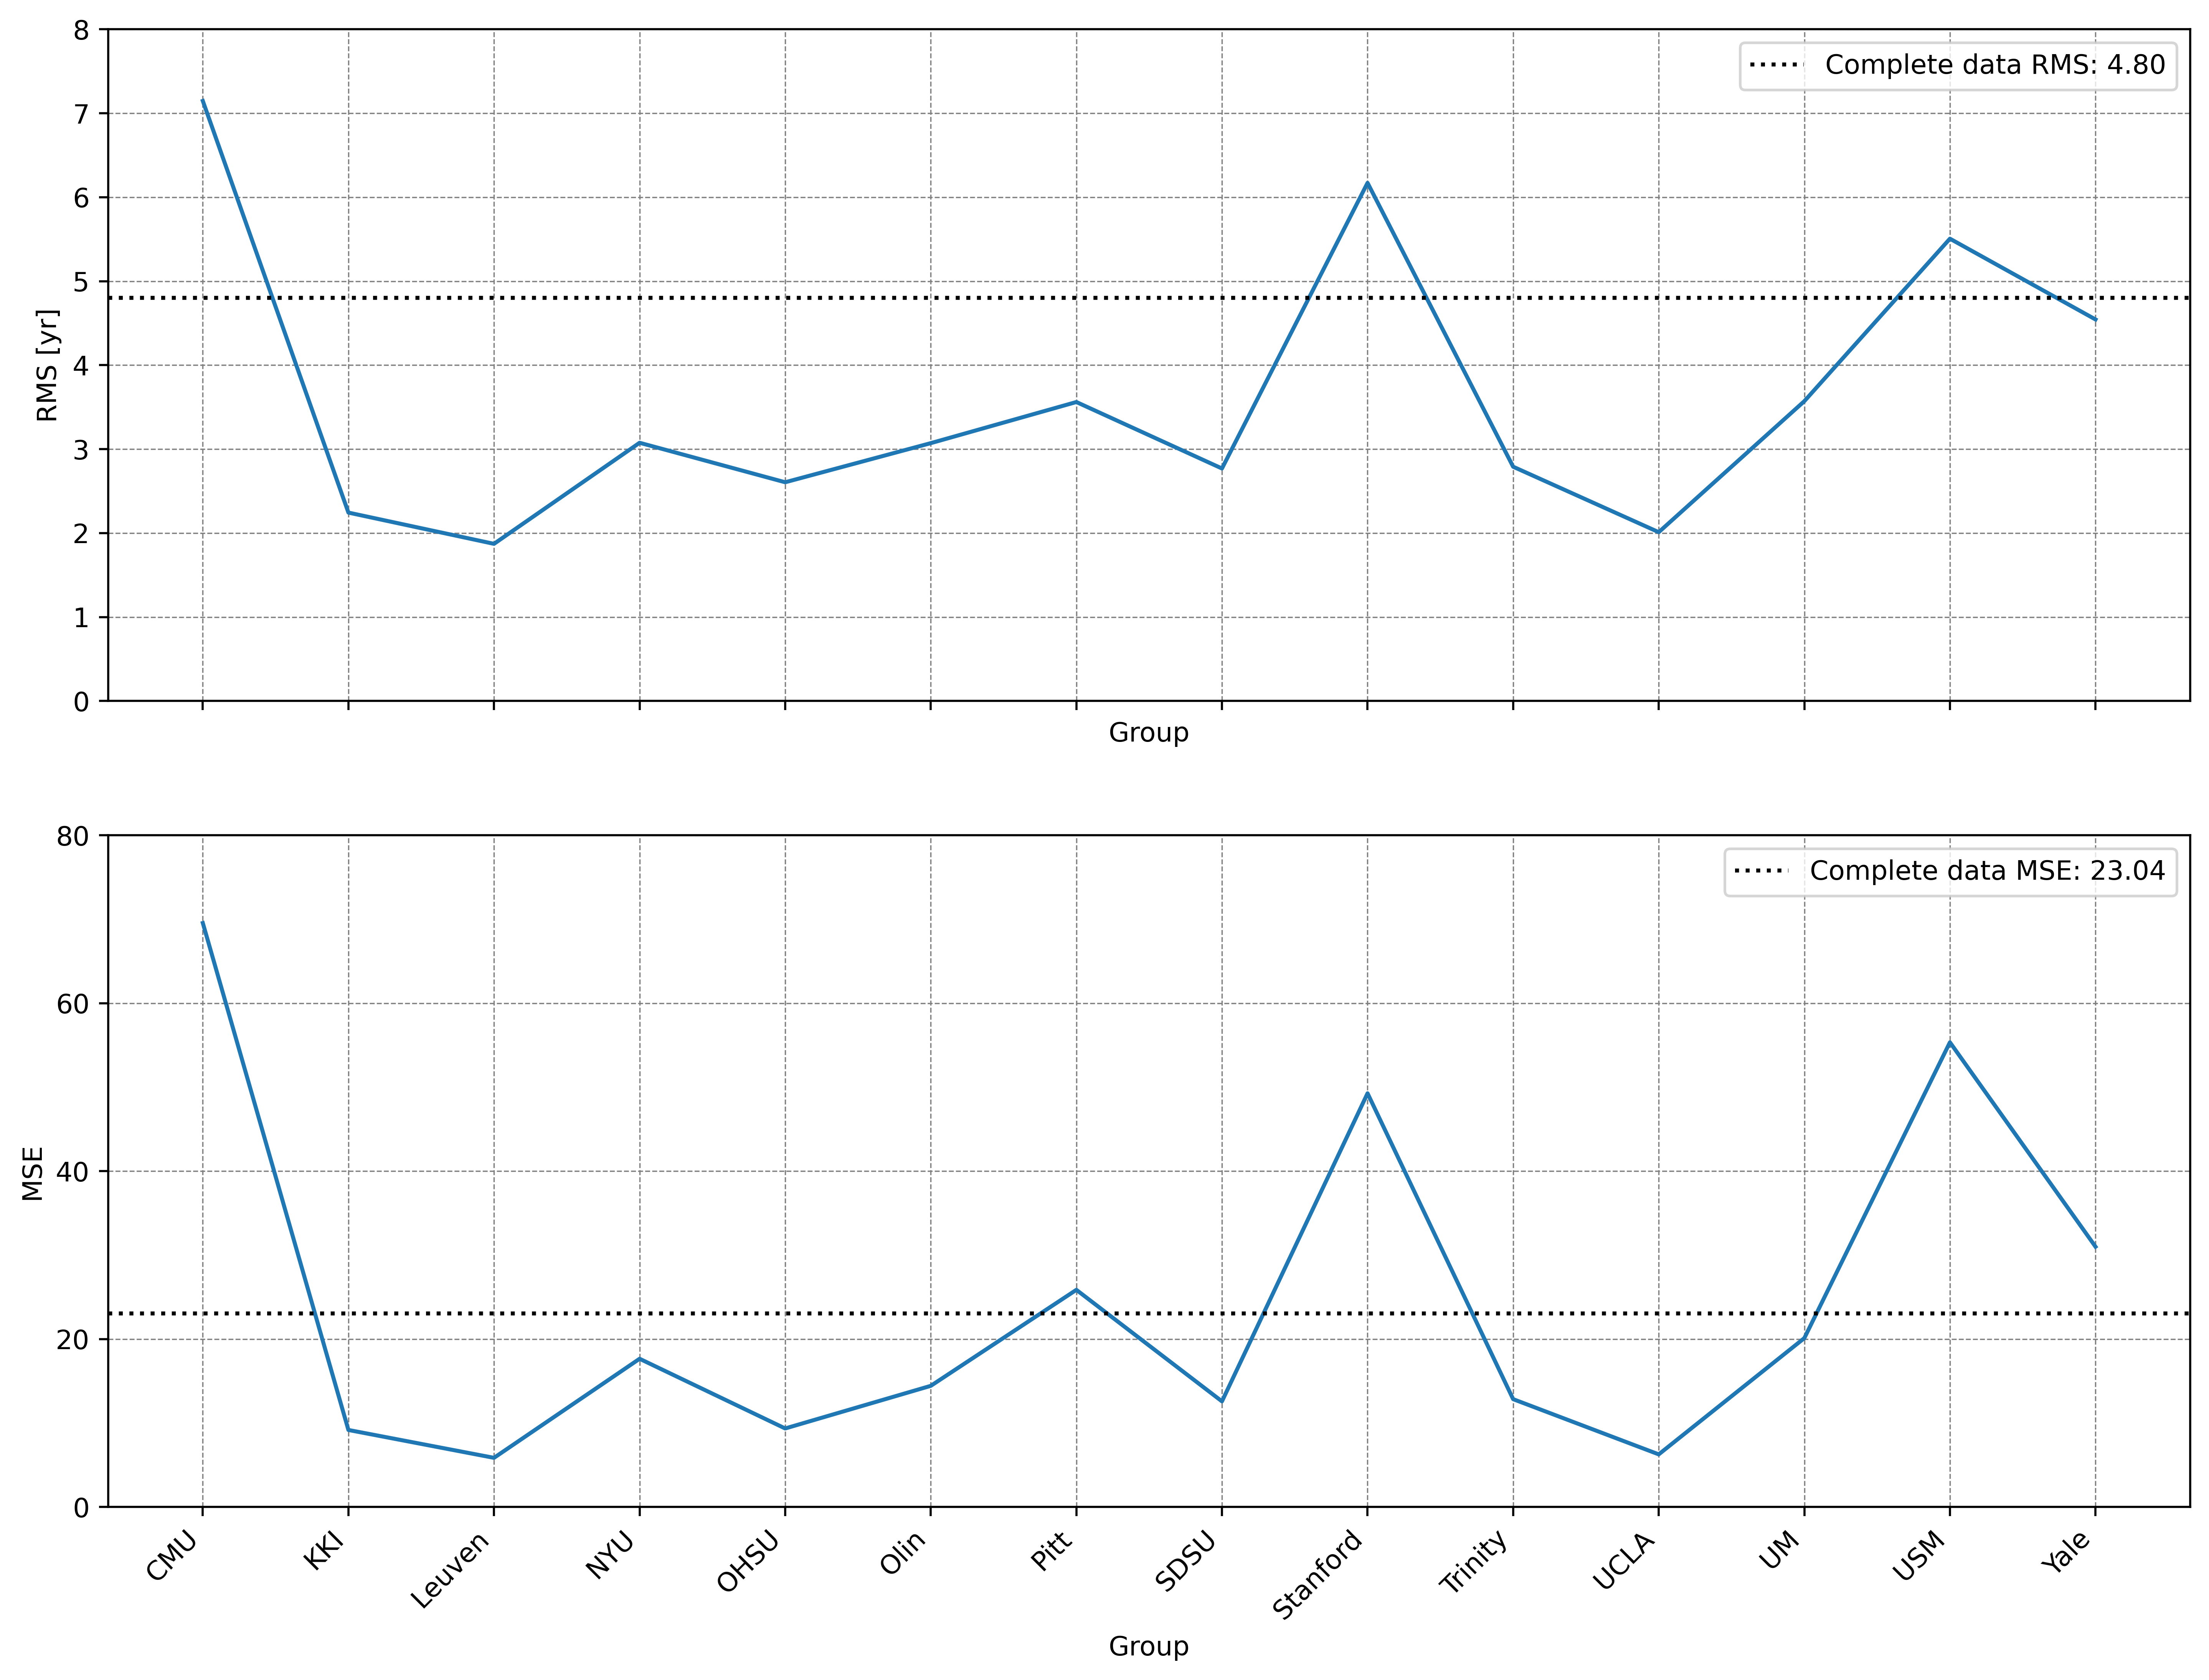
\includegraphics[width=0.8\textwidth]{result_without_out.png}
\captionof{figure}{Prestazione del modello allenato senza i tre gruppi a maggiore errore sui soli gruppi a basso errore.}
\end{figure}
\begin{figure}
	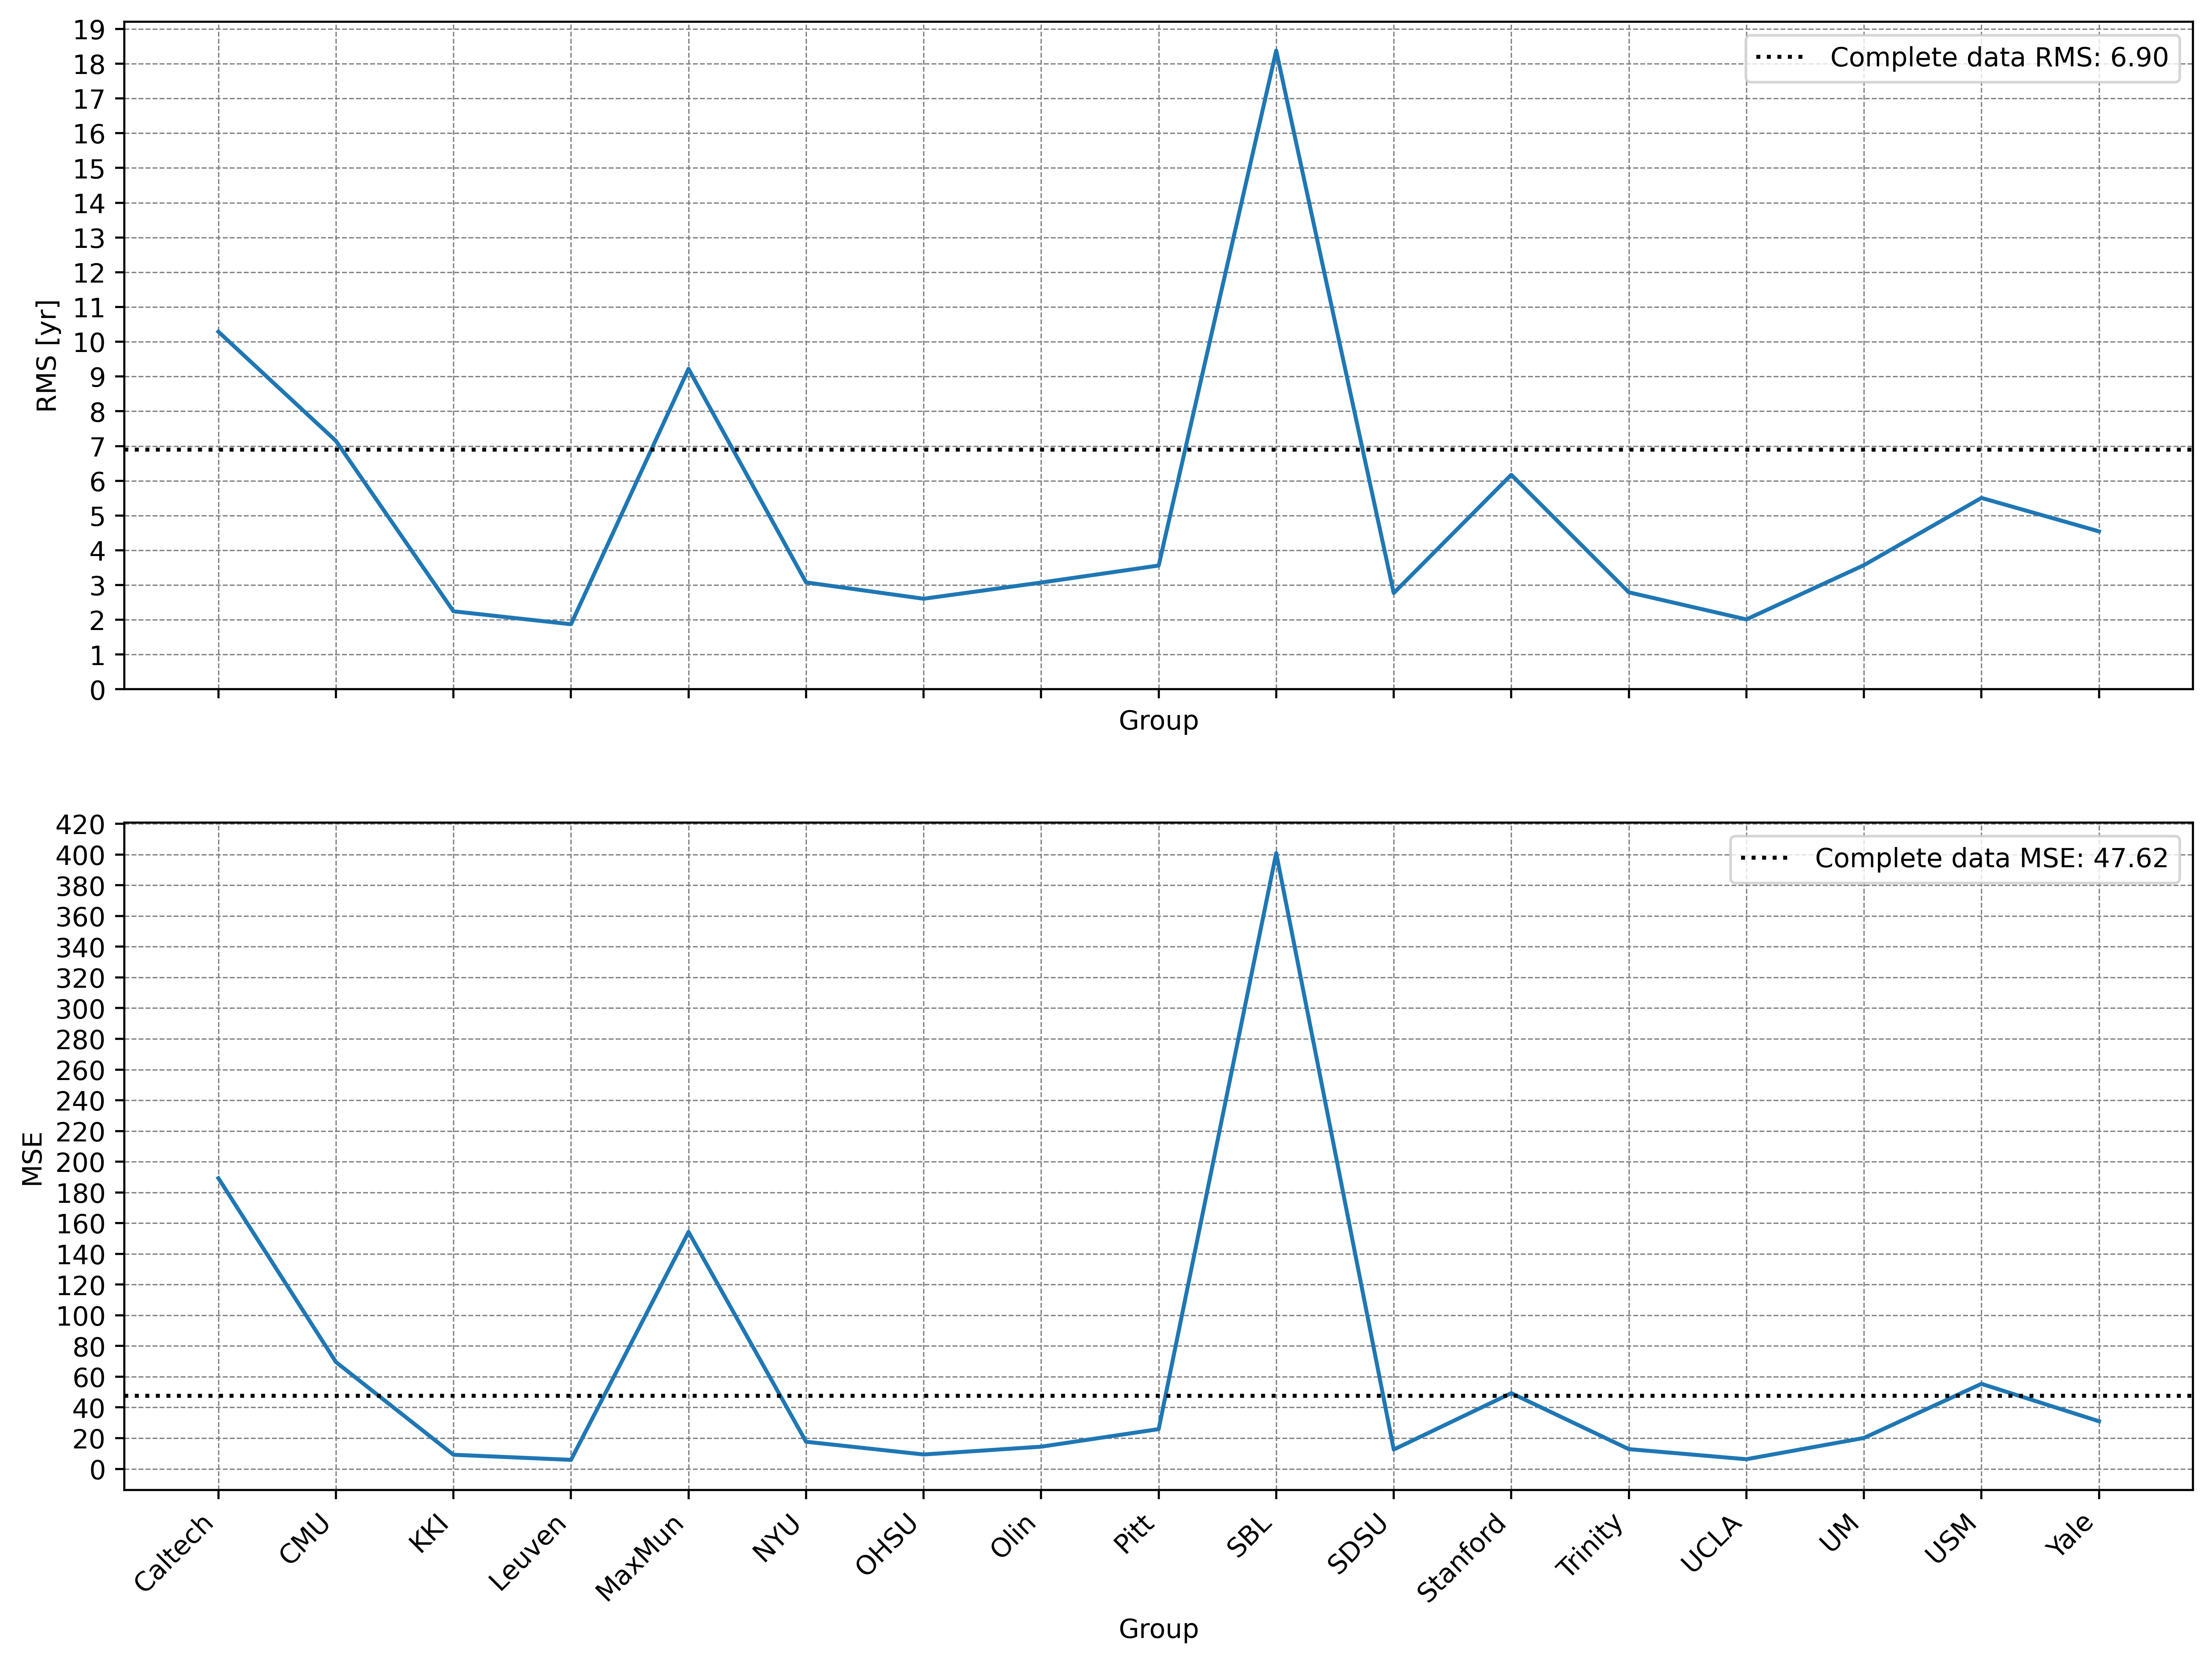
\includegraphics[width=0.8\textwidth]{result_without_out_overall.png}
\captionof{figure}{Prestazione del modello allenato con e senza i tre gruppi a maggiore errore.}
\end{figure}






\section*{Appendice}

Il progetto utilizza un repository pubblico su GitHub. 

Ha un ramo principale e tre rami attivi: develop, feature/docs e feature/presentation.




La documentazione del progetto è stata generata tramite Sphinx, utilizzando la sua funzionalità \emph{autodoc} per estrarre le docstring dal codice sorgente.

Il repository pubblico su GitHub consente di distribuire la documentazione del progetto attraverso ReadTheDocs e le Pages di GitHub.







\end{document}
